% move all configuration stuff into one file so we can focus on the content
\documentclass[aspectratio=169,hyperref={pdfpagelabels=false,colorlinks=true,linkcolor=white,urlcolor=lightblue},xcolor={table},t]{beamer}

%%%%%%%%%%%%%%%%%%%%%%%%%%%%%%%%%%%%%%%%%%%%%%%%%%%%%%%%%%%%%%%%%%%%%%%%%%%%%%%%%%
%%%%%%%%%%%%%%%%%%%%%%%%%%%%%%%%%%%%%%%%%%%%%%%%%%%%%%%%%%%%%%%%%%%%%%%%%%%%%%%%%%
% packages
\usepackage{pict2e}
\usepackage{epic}
\usepackage{amsmath,amsfonts,amssymb}
\usepackage{units}
\usepackage{fancybox}
\usepackage[absolute,overlay]{textpos} 
%\usepackage[table]{xcolor}
\usepackage{animate}
\usepackage{gensymb}
%\usepackage{graphicx}
%\usepackage{longtable}
\usepackage{multirow}
\usepackage{silence}
\usepackage{tikz}
\usepackage[backend=bibtex,style=ieee]{biblatex}
\AtEveryCitekey{\iffootnote{\tiny}{}}
%\addbibresource{include/references}



% fontsize
\let\Tiny=\tiny

%%%%%%%%%%%%%%%%%%%%%%%%%%%%%%%%%%%%%%%%%%%%%%%%%%%%%%%%%%%%%%%%%%%%%%%%%%%%%%%%%%
%%%%%%%%%%%%%%%%%%%%%%%%%%%%%%%%%%%%%%%%%%%%%%%%%%%%%%%%%%%%%%%%%%%%%%%%%%%%%%%%%%
% warnings
\pdfsuppresswarningpagegroup=1
\WarningFilter{biblatex}{Patching footnotes failed}
\WarningFilter{latexfont}{Font shape}
\WarningFilter{latexfont}{Some font shapes}
\WarningFilter{gensymb}{Not defining}


%%%%%%%%%%%%%%%%%%%%%%%%%%%%%%%%%%%%%%%%%%%%%%%%%%%%%%%%%%%%%%%%%%%%%%%%%%%%%%%%%%
%%%%%%%%%%%%%%%%%%%%%%%%%%%%%%%%%%%%%%%%%%%%%%%%%%%%%%%%%%%%%%%%%%%%%%%%%%%%%%%%%%
% theme & layout
\usetheme{Frankfurt}
\useinnertheme{rectangles}


%%%%%%%%%%%%%%%%%%%%%%%%%%%%%%%%%%%%%%%%%%%%%%%%%%%%%%%%%%%%%%%%%%%%%%%%%%%%%%%%%%
\setbeamertemplate{frametitle}[default][colsep=-4bp,rounded=false,shadow=false]
\setbeamertemplate{frametitle}
{%
    \nointerlineskip%
    %\vskip-0.5ex
    \begin{beamercolorbox}[wd=\paperwidth,ht=3.5ex,dp=0.6ex]{frametitle}
        \hspace*{1.3ex}\insertframetitle%
        
        \hspace*{1.3ex}\small\insertframesubtitle%
    \end{beamercolorbox}%
    \begin{textblock*}{100mm}(13.75cm,1cm)
        
\includegraphics[height=.4cm,keepaspectratio]{../shared/Logo_GTCMT_white}
    \end{textblock*}
}


%%%%%%%%%%%%%%%%%%%%%%%%%%%%%%%%%%%%%%%%%%%%%%%%%%%%%%%%%%%%%%%%%%%%%%%%%%%%%%%%%%
\setbeamertemplate{title page}[default][colsep=-4bp,rounded=false,shadow=false]
\setbeamertemplate{title page}
{
    %\begin{textblock*}{100mm}(15cm,.51cm)
            %\href{https://github.com/alexanderlerch/ACA-Slides/blob/2nd_edition/\jobname.pdf}{\includegraphics[height=.5cm,keepaspectratio]{graph/Logo_github}}\hspace*{2ex}
    %\end{textblock*}
    %\begin{textblock*}{100mm}(15cm,1.3cm)
            %\href{\IEEELink}{\includegraphics[height=.5cm,keepaspectratio]{graph/icon/book}}\hspace*{2ex}
    %\end{textblock*}
    \vskip-10ex
    \begin{beamercolorbox}[wd=\paperwidth,ht=.7\paperheight,dp=0.6ex]{frametitle} %35ex
        %\begin{flushright}
            %\href{http://www.gtcmt.gatech.edu}{
\includegraphics[height=.8cm,keepaspectratio]{graph/Logo_GTCMT_black}}\hspace*{2ex}
        %\end{flushright}
        
        \hspace*{1.8ex}\LARGE\inserttitle%
        
        \vspace*{.5ex}
        
        \hspace*{1.3ex}\small\insertsubtitle%
        
        \vspace*{.5ex}
    \end{beamercolorbox}%
    \nointerlineskip%
    \begin{beamercolorbox}[wd=\paperwidth,ht=.4\paperheight,dp=0.6ex]{page number in head/foot}
        %\vspace*{-.5ex}
        \hspace*{1.7ex}\small\insertauthor%
        
        %\hspace*{1.7ex}\small }%
        
        \vspace*{12ex}
        \vfill
        \begin{flushright}
            \href{http://www.gtcmt.gatech.edu}{
\includegraphics[height=.5cm,keepaspectratio]{../shared/Logo_GTCMT_black}}\hspace*{2ex}
        \end{flushright}
    \end{beamercolorbox}%
}


%%%%%%%%%%%%%%%%%%%%%%%%%%%%%%%%%%%%%%%%%%%%%%%%%%%%%%%%%%%%%%%%%%%%%%%%%%%%%%%%%%
%\makeatother
\setbeamertemplate{footline}
{
  \leavevmode%
  \hbox{%
  \begin{beamercolorbox}[wd=.5\paperwidth,ht=2.25ex,dp=1ex,left,leftskip=1ex]{page number in head/foot}%
    \insertsubtitle
  \end{beamercolorbox}%
  \begin{beamercolorbox}[wd=.5\paperwidth,ht=2.25ex,dp=1ex,right,rightskip=1ex]{page number in head/foot}%
    \hfill
    \insertframenumber{} / \inserttotalframenumber
  \end{beamercolorbox}}%
  \vskip0pt%
}
%\makeatletter


%%%%%%%%%%%%%%%%%%%%%%%%%%%%%%%%%%%%%%%%%%%%%%%%%%%%%%%%%%%%%%%%%%%%%%%%%%%%%%%%%%
\beamertemplatenavigationsymbolsempty
\setbeamertemplate{navigation symbols}{}
\setbeamertemplate{blocks}[default]%[rounded=false,shadow=false]
\setbeamertemplate{itemize item}[square]
\setbeamertemplate{itemize subitem}[circle]
\setbeamertemplate{itemize subsubitem}[triangle]
\setbeamertemplate{enumerate item}[square]
\setbeamertemplate{enumerate subitem}[circle]
\setbeamertemplate{enumerate subsubitem}[circle]


%%%%%%%%%%%%%%%%%%%%%%%%%%%%%%%%%%%%%%%%%%%%%%%%%%%%%%%%%%%%%%%%%%%%%%%%%%%%%%%%%%
% colors
\setbeamercolor{structure}{fg=darkgray}
\setbeamercovered{transparent} %invisible
\setbeamercolor{bibliography entry author}{fg=black}
\setbeamercolor*{bibliography entry title}{fg=black}
\setbeamercolor*{bibliography entry note}{fg=black}
\setbeamercolor{frametitle}{fg=black}
\setbeamercolor{title}{fg=white}
\setbeamercolor{subtitle}{fg=white}
\setbeamercolor{frametitle}{fg=white}
\setbeamercolor{framesubtitle}{fg=white}
\setbeamercolor{mini frame}{fg=white, bg=black}
\setbeamercolor{section in head/foot}{fg=white, bg=darkgray}
\setbeamercolor{page number in head/foot}{fg=black, bg=gtgold}
\setbeamercolor{item projected}{fg=white, bg=black}

%---------------------------------------------------------------------------------

%%%%%%%%%%%%%%%%%%%%%%%%%%%%%%%%%%%%%%%%%%%%%%%%%%%%%%%%%%%%%%%%%%%%%%%%%%%%%%%%%%
%%%%%%%%%%%%%%%%%%%%%%%%%%%%%%%%%%%%%%%%%%%%%%%%%%%%%%%%%%%%%%%%%%%%%%%%%%%%%%%%%%
% title information
\title[]{MUSI6202: Digital Signal Processing for Music}   
\author[alexander lerch]{alexander lerch} 
%\institute{~}
%\date[Alexander Lerch]{}
%\titlegraphic{\vspace{-16mm}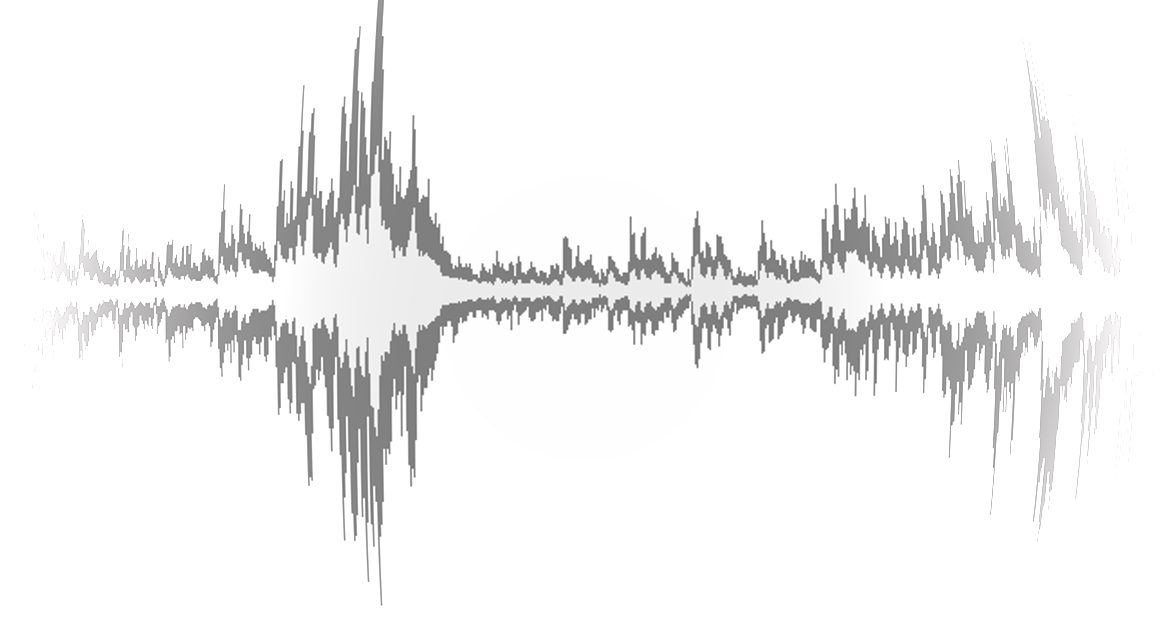
\includegraphics[width=\textwidth,height=3cm]{title}}

%%%%%%%%%%%%%%%%%%%%%%%%%%%%%%%%%%%%%%%%%%%%%%%%%%%%%%%%%%%%%%%%%%%%%%%%%%%%%%%%%%
%%%%%%%%%%%%%%%%%%%%%%%%%%%%%%%%%%%%%%%%%%%%%%%%%%%%%%%%%%%%%%%%%%%%%%%%%%%%%%%%%%
% colors
\definecolor{gtgold}{rgb}{.914, .664, 0} %0e7eed {rgb}{0.88,0.66,1,0.06} [234, 170, 0]/256 %96caff
\definecolor{darkgray}{rgb}{.15, .15, .15}
\definecolor{lightblue}{HTML}{0e7eed}
\definecolor{highlight}{rgb}{0, 0, 1} %_less!40

%%%%%%%%%%%%%%%%%%%%%%%%%%%%%%%%%%%%%%%%%%%%%%%%%%%%%%%%%%%%%%%%%%%%%%%%%%%%%%%%%%
%%%%%%%%%%%%%%%%%%%%%%%%%%%%%%%%%%%%%%%%%%%%%%%%%%%%%%%%%%%%%%%%%%%%%%%%%%%%%%%%%%
% relative paths
\graphicspath{{../graph/}}


%%%%%%%%%%%%%%%%%%%%%%%%%%%%%%%%%%%%%%%%%%%%%%%%%%%%%%%%%%%%%%%%%%%%%%%%%%%%%%%%%%
%%%%%%%%%%%%%%%%%%%%%%%%%%%%%%%%%%%%%%%%%%%%%%%%%%%%%%%%%%%%%%%%%%%%%%%%%%%%%%%%%%
% units
\setlength{\unitlength}{1mm}

%%%%%%%%%%%%%%%%%%%%%%%%%%%%%%%%%%%%%%%%%%%%%%%%%%%%%%%%%%%%%%%%%%%%%%%%%%%%%%%%%%
%%%%%%%%%%%%%%%%%%%%%%%%%%%%%%%%%%%%%%%%%%%%%%%%%%%%%%%%%%%%%%%%%%%%%%%%%%%%%%%%%%
% math
\DeclareMathOperator*{\argmax}{argmax}
\DeclareMathOperator*{\argmin}{argmin}
\DeclareMathOperator*{\atan}{atan}
\DeclareMathOperator*{\arcsinh}{arcsinh}
\DeclareMathOperator*{\sign}{sign}
\DeclareMathOperator*{\tcdf}{tcdf}
\DeclareMathOperator*{\si}{sinc}
\DeclareMathOperator*{\princarg}{princarg}
\DeclareMathOperator*{\arccosh}{arccosh}
\DeclareMathOperator*{\hwr}{HWR}
\DeclareMathOperator*{\flip}{flip}
\DeclareMathOperator*{\sinc}{sinc}
\DeclareMathOperator*{\floor}{floor}
\newcommand{\e}{{e}}
\newcommand{\jom}{\mathrm{j}\omega}
\newcommand{\jOm}{\mathrm{j}\Omega}
\newcommand   {\mat}[1]    		{\boldsymbol{\uppercase{#1}}}		%bold
\renewcommand {\vec}[1]    		{\boldsymbol{\lowercase{#1}}}		%bold

%%%%%%%%%%%%%%%%%%%%%%%%%%%%%%%%%%%%%%%%%%%%%%%%%%%%%%%%%%%%%%%%%%%%%%%%%%%%%%%%%%
%%%%%%%%%%%%%%%%%%%%%%%%%%%%%%%%%%%%%%%%%%%%%%%%%%%%%%%%%%%%%%%%%%%%%%%%%%%%%%%%%%
% media9
\newcommand{\includeaudio}[1]{
\href{run:audio/#1.mp3}{
\includegraphics[width=5mm, height=5mm]{graph/SpeakerIcon}}}

\newcommand{\includeanimation}[4]{{\begin{center}
                        \animategraphics[autoplay,loop,scale=.7]{#4}{animation/#1-}{#2}{#3}        
                        \end{center}
                        \addreference{matlab source: \href{https://github.com/alexanderlerch/ACA-Plots/blob/master/matlab/animate#1.m}{matlab/animate#1.m}}}
                        \inserticon{video}}
                        
%%%%%%%%%%%%%%%%%%%%%%%%%%%%%%%%%%%%%%%%%%%%%%%%%%%%%%%%%%%%%%%%%%%%%%%%%%%%%%%%%%
%%%%%%%%%%%%%%%%%%%%%%%%%%%%%%%%%%%%%%%%%%%%%%%%%%%%%%%%%%%%%%%%%%%%%%%%%%%%%%%%%%
% other commands
\newcommand{\question}[1]{%\vspace{-4mm}
                          \setbeamercovered{invisible}
                          \begin{columns}[T]
                            \column{.9\textwidth}
                                \textbf{#1}
                            \column{.1\textwidth}
                                \vspace{-8mm}
                                \begin{flushright}
                                     
\includegraphics[width=.9\columnwidth]{graph/question_mark}
                                \end{flushright}
                                \vspace{6mm}
                          \end{columns}\pause\vspace{-12mm}}

\newcommand{\toremember}[1]{
                        \inserticon{lightbulb}
                        }

\newcommand{\matlabexercise}[1]{%\vspace{-4mm}
                          \setbeamercovered{invisible}
                          \begin{columns}[T]
                            \column{.8\textwidth}
                                \textbf{matlab exercise}: #1
                            \column{.2\textwidth}
                                \begin{flushright}
                                     \includegraphics[scale=.5]{graph/logo_matlab}
                                \end{flushright}
                                %\vspace{6mm}
                          \end{columns}}

\newcommand{\addreference}[1]{  
                  
                    \begin{textblock*}{\baselineskip }(.98\paperwidth,.5\textheight) %(1.15\textwidth,.4\textheight)
                         \begin{minipage}[b][.5\paperheight][b]{1cm}%
                            \vfill%
                             \rotatebox{90}{\tiny {#1}}
                        \end{minipage}
                   \end{textblock*}
                    }
                    
\newcommand{\figwithmatlab}[1]{
                    \begin{figure}
                        \centering
                        \includegraphics[scale=.7]{#1}
                        %\label{fig:#1}
                    \end{figure}
                    
                    \addreference{matlab source: \href{https://github.com/alexanderlerch/MUSI-6202/blob/main/matlab/plot#1.m}{plot#1.m}}}
\newcommand{\figwithref}[2]{
                    \begin{figure}
                        \centering
                        \includegraphics[scale=.7]{#1}
                        \label{fig:#1}
                    \end{figure}
                    
                    \addreference{#2}}  
                                    
\newcommand{\inserticon}[1]{
                    \begin{textblock*}{100mm}(14.5cm,7.5cm)
                        \includegraphics[height=.8cm,keepaspectratio]{graph/#1}
                    \end{textblock*}}            

%%%%%%%%%%%%%%%%%%%%%%%%%%%%%%%%%%%%%%%%%%%%%%%%%%%%%%%%%%%%%%%%%%%%%%%%%%%%%%%%%%
%%%%%%%%%%%%%%%%%%%%%%%%%%%%%%%%%%%%%%%%%%%%%%%%%%%%%%%%%%%%%%%%%%%%%%%%%%%%%%%%%%
% counters
\newcounter{i}
\newcounter{j}
\newcounter{iXOffset}
\newcounter{iYOffset}
\newcounter{iXBlockSize}
\newcounter{iYBlockSize}
\newcounter{iYBlockSizeDiv2}
\newcounter{iXBlockSizeDiv2}
\newcounter{iDistance}

\newcommand{\IEEELink}{https://ieeexplore.ieee.org/servlet/opac?bknumber=9965970}

\addbibresource{../shared/references}



\subtitle{Part 14: Improving (Re-)Quantization Quality}

%%%%%%%%%%%%%%%%%%%%%%%%%%%%%%%%%%%%%%%%%%%%%%%%%%%%%%%%%%%%%%%%%%%%%%%%%%%%
\begin{document}
    % generate title page
	\title[]{Digital Signal Processing for Music}   
\author[alexander lerch]{alexander lerch} 
%\institute{~}
%\date[Alexander Lerch]{}
\titlegraphic{\vspace{-16mm}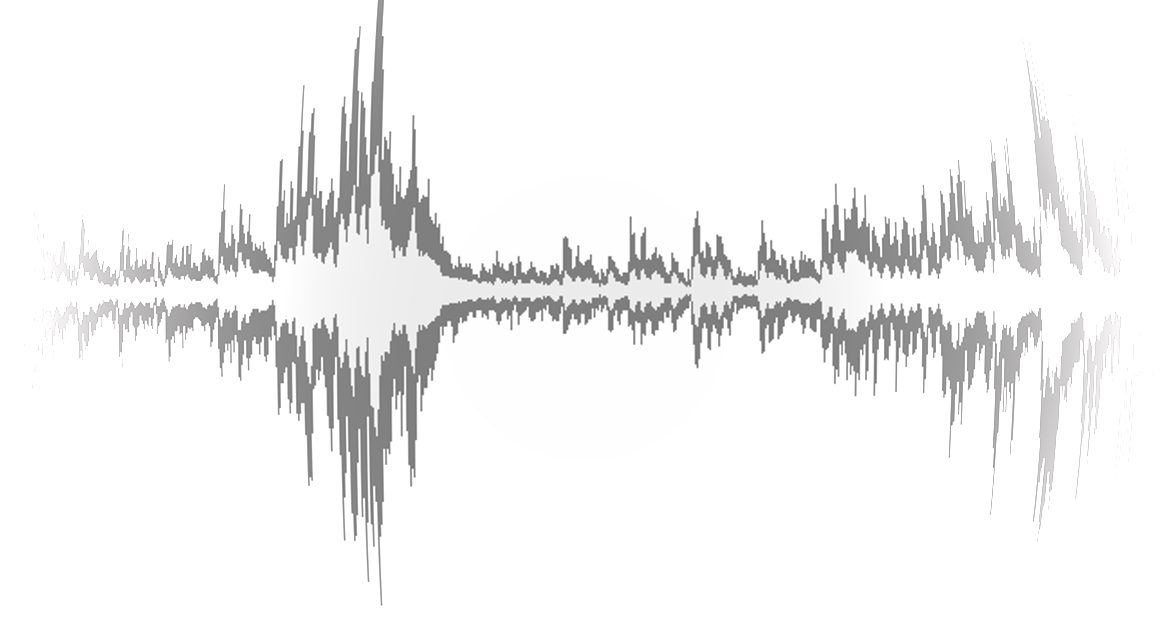
\includegraphics[width=\textwidth,height=3cm]{title}}


\begin{frame}
    \titlepage
    %\vspace{-5mm}
    \begin{flushright}
        \href{http://www.gtcmt.gatech.edu}{
\includegraphics[height=.8cm,keepaspectratio]{../shared/Logo_GTCMT_black}}
    \end{flushright}
\end{frame}


\section[intro]{introduction}
	\begin{frame}{introduction}{introduction}
        \question{Quantization error properties are fixed, so there is no way of improving the quality. Is there??}
        
        \bigskip
        we will discuss three ways of ``cheating'' for better quality
        \begin{itemize}
            \item   of quantization:
                \begin{itemize}
                    \item   oversampling
                    \item   noise-shaping
                \end{itemize}
            \smallskip
            \item   of re-quantization/ word length reduction
                \begin{itemize}
                    \item   dither
                    \item   noise shaping
                \end{itemize}
        \end{itemize}
    \end{frame}
\section{oversampling}

	\begin{frame}{oversampling}{introduction}
		\begin{itemize}
            \item   \textbf{oversampling}: 
            \begin{itemize}
                \item<2->[$\Rightarrow$]	less steep anti-aliasing filters
                \item<2->[$\Rightarrow$]	other advantages?
            \end{itemize}

            \bigskip
			\item<3->	remember \textbf{quantization error properties}
			\begin{enumerate}
				\item	\textit{white} noise: flat spectrum
				\item	overall noise power: constant (same for high or low sample rates)
                \bigskip
                \item<4->[$\Rightarrow$] $|Q(\jom)|^2 \sim \frac{\Delta^2}{12\cdot \omega_\mathrm{S}}$
			\end{enumerate}
		\end{itemize}
        
        \bigskip
        \only<5>{
        \question{can oversampling take advantage of these properties to \textit{reduce quantization error power }}
        }
	\end{frame}	
    
	\begin{frame}{oversampling}{visualization}
        \vspace{-8mm}
        \begin{columns}
        \column{.5\linewidth}
		\begin{figure}
			\centering
				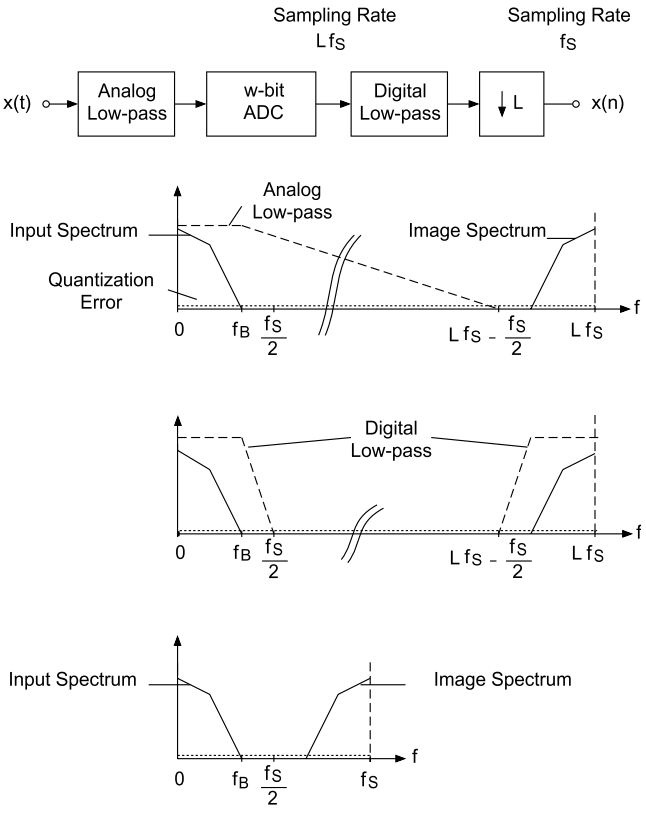
\includegraphics[scale=.32]{Graph/oversampling2}
		\end{figure}
        \column{.5\linewidth}
		\figwithmatlab{Oversampling}
        \end{columns}
	\end{frame}	
	\begin{frame}{oversampling}{SNR gain}
		\begin{eqnarray*}
			\omega^\ast_S &=& L\cdot \omega_S\\
            \bigskip
			|Q(\jom)|^2 &=& \frac{\Delta^2}{12\cdot \omega^\ast_S}\\
			&=& \frac{\Delta^2}{12\cdot L\cdot \omega_S}\\
			\pause
            \bigskip
			W^\ast_\mathrm{Q,LP} &=& \frac{\Delta^2}{12\cdot L}\\
			\pause
            \bigskip
            \Rightarrow&&\\
			SNR^\ast &=& \only<3>{?}\only<4->{6.02\cdot w + 10\log_{10} (L) + c_S}
		\end{eqnarray*}
	\end{frame}	
	\begin{frame}{oversampling}{summary}
		\toremember{}
		\begin{block}{\textbf{oversampling}}
			\centering
			\begin{equation*}
				SNR = 6.02\cdot w + c_{\mathrm{S}} + {\color{gtgold}{10\cdot\log_{10}(L)}}\quad [dB]
			\end{equation*}
			\begin{itemize}
				\item	every doubling of $f_{\mathrm{S}}$ adds app.\ \unit[3]{dB} SNR
			\end{itemize}
		\end{block}
	\end{frame}	
        
\section{dither}
	\begin{frame}{dither}{introduction 1/2}
        \begin{columns}
            \column{.5\textwidth}
		\begin{itemize}
			\item	previous assumption:\\ \textbf{quantization error is white noise} (rect)
				\pause
				\begin{itemize}
					\item[$\rightarrow$]	\textbf{no correlation} between signal and quantization error
				\end{itemize}
                \smallskip
			\visible<2->{
			\item	\textbf{not true for}
				\begin{itemize}
					\item	low signal level
					\item	low signal frequency
				\end{itemize}
			}
            \visible<3->{
                \smallskip
             \item	\textbf{solution}:
				\begin{itemize}
					\item	 \textbf{add noise before quantization: dither}
				\end{itemize}
                }
		\end{itemize}
        \column{0.5\textwidth}
			\visible<2->{
      	\figwithmatlab{SineQuant}
        }
    \end{columns}
	\end{frame}	
	\begin{frame}{dither}{introduction 2/2}
		\vspace{-5mm}
        \figwithmatlab{Dither}
	\end{frame}	
	\begin{frame}{dither}{process}
		\begin{figure}
			\centering
				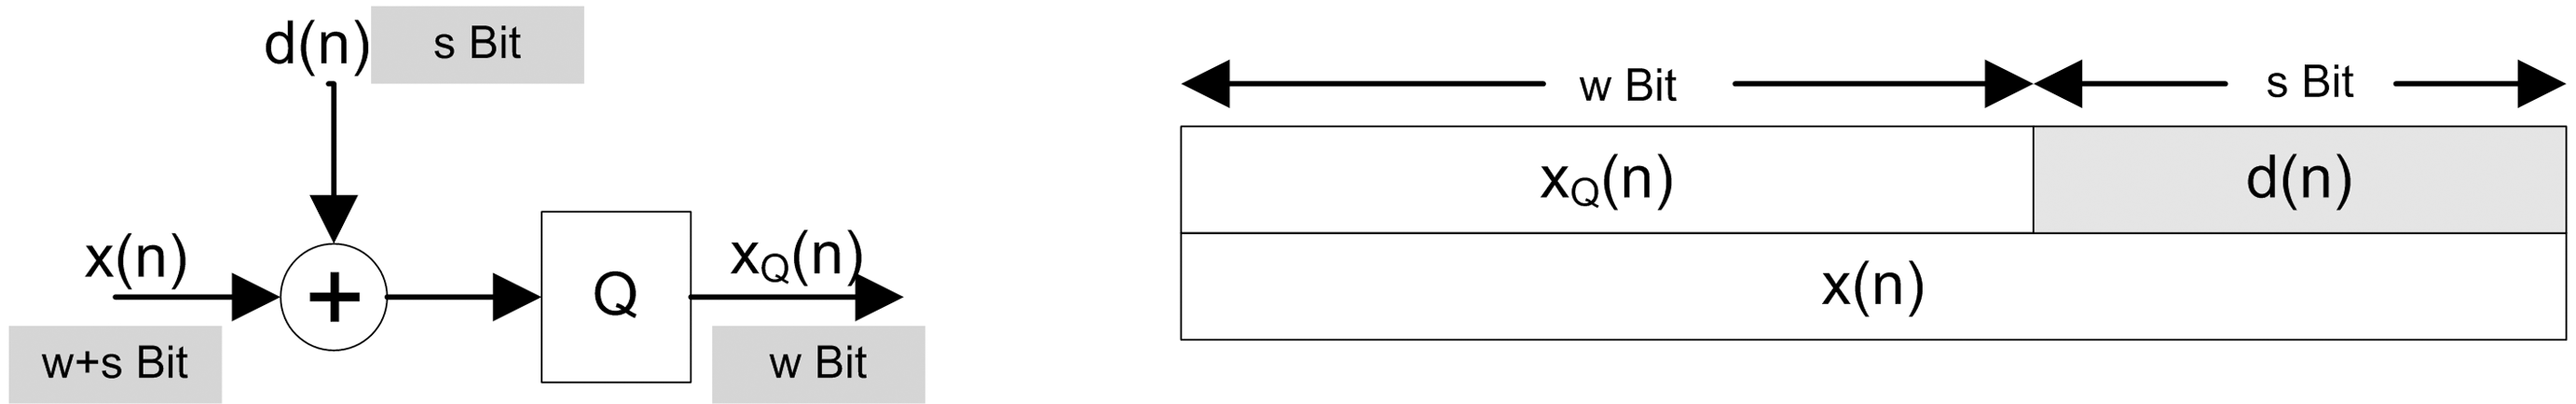
\includegraphics[scale=0.9]{Graph/quantisierung_mit_dither.png}
		\end{figure}
	\end{frame}	
	\begin{frame}{dither}{simple example}
		input signal: DC at $1.3\cdot\Delta$
        \bigskip
		\begin{itemize}
			\item	\textbf{w/o dither}: 
				\begin{itemize}
					\item	output value: $\Delta$
					\item	\textit{quantization error constant}: $.3\cdot\Delta$
				\end{itemize}
			\pause
            \bigskip
			\item	\textbf{w/ dither ($-\Delta/2\ldots\Delta/2$)}: 
				\begin{itemize}
					\item	signal is most frequently quantized to $\Delta$ ($p = 0.7$), but sometimes to $2\cdot\Delta$ ($p=0.3$)
					\bigskip
                    \item<3->	\textit{average} output value: $1.3\cdot\Delta$!
                    \item<3->   \textit{quantization error varying} between $0.3\cdot\Delta$ and $0.7\cdot\Delta$
				\end{itemize}
		\end{itemize}
	\end{frame}	
	\begin{frame}{dither}{properties}
		\begin{figure}
			\centering
				%\begin{footnotesize}
    \begin{picture}(85,20)
        \setcounter{iXOffset}{0}
        \setcounter{iYOffset}{0}
        \setcounter{iXBlockSize}{10}
        \setcounter{iXBlockSizeDiv2}{5}
        \setcounter{iYBlockSize}{10}
        \setcounter{iYBlockSizeDiv2}{5}
        \setcounter{iDistance}{10}

    \addtocounter{iYOffset}{\value{iYBlockSizeDiv2}}

    \put(\value{iXOffset}, \value{iYOffset})
        {\vector(1,0){\value{iDistance}}}

    \addtocounter{iYOffset}{1}
    \put(\value{iXOffset}, \value{iYOffset})
        {\text{$x(i)$}}
    \addtocounter{iYOffset}{-1}

    \addtocounter{iXOffset}{\value{iDistance}}
    \addtocounter{iXOffset}{2}
    \put(\value{iXOffset}, \value{iYOffset})
        {\circle{4}} 
    \addtocounter{iXOffset}{-1}
    \addtocounter{iYOffset}{-1}
    \put(\value{iXOffset}, \value{iYOffset})
        {\text{\large{+}}}
    \addtocounter{iXOffset}{1}
    \addtocounter{iYOffset}{1}
        

    %\addtocounter{iXOffset}{2}
    \addtocounter{iYOffset}{\value{iDistance}}
    \addtocounter{iYOffset}{2}
    \put(\value{iXOffset}, \value{iYOffset})
        {\vector(0,-1){\value{iDistance}}}
    \addtocounter{iYOffset}{-\value{iDistance}}
    \addtocounter{iYOffset}{-2}
    \addtocounter{iXOffset}{2}
    \put(\value{iXOffset}, \value{iYOffset})
        {\vector(1,0){\value{iDistance}}}

    \addtocounter{iYOffset}{\value{iDistance}}
    \addtocounter{iYOffset}{-1}
    \addtocounter{iXOffset}{-1}
    \put(\value{iXOffset}, \value{iYOffset})
        {\text{$d(i)$}}
    \addtocounter{iXOffset}{1}
    \addtocounter{iYOffset}{-\value{iDistance}}
    \addtocounter{iYOffset}{1}

    \addtocounter{iYOffset}{-\value{iYBlockSizeDiv2}}
    \addtocounter{iXOffset}{\value{iDistance}}
    \put(\value{iXOffset}, \value{iYOffset})
        {\framebox(\value{iXBlockSize}, \value{iYBlockSize}) {Q}}

    \addtocounter{iXOffset}{\value{iXBlockSize}}
    \addtocounter{iYOffset}{\value{iYBlockSizeDiv2}}

    \put(\value{iXOffset}, \value{iYOffset})
        {\vector(1,0){\value{iDistance}}}

    \addtocounter{iXOffset}{3}
    \addtocounter{iYOffset}{1}
    \put(\value{iXOffset}, \value{iYOffset})
        {\text{$x_\mathrm{Q}(i)$}}
    \addtocounter{iYOffset}{-1}
    \addtocounter{iXOffset}{-3}
 
    \addtocounter{iXOffset}{\value{iXBlockSize}}
    \addtocounter{iXOffset}{\value{iXBlockSize}}
    \setcounter{iYOffset}{0}

    \put(\value{iXOffset}, \value{iYOffset})
        {\framebox(60, \value{iYBlockSizeDiv2}) {$x(i)$}}

    \addtocounter{iYOffset}{\value{iYBlockSizeDiv2}}
    \put(\value{iXOffset}, \value{iYOffset})
        {\framebox(40, \value{iYBlockSizeDiv2}) {$x_\mathrm{Q}(i)$}}
    \addtocounter{iXOffset}{40}
    \put(\value{iXOffset}, \value{iYOffset})
        {\framebox(20, \value{iYBlockSizeDiv2}) {$d(i)$}}

    \addtocounter{iYOffset}{\value{iYBlockSizeDiv2}}
    \addtocounter{iYOffset}{1}
    \addtocounter{iXOffset}{-40}
    \addtocounter{iXOffset}{16}
    \put(\value{iXOffset}, \value{iYOffset})
        {\vector(-1,0){16}}
    \addtocounter{iXOffset}{2}
    %\addtocounter{iYOffset}{-1}
    \put(\value{iXOffset}, \value{iYOffset})
        {\text{\tiny{\unit[w]{Bit}}}}
    \addtocounter{iXOffset}{-2}
    \addtocounter{iXOffset}{8}
    \put(\value{iXOffset}, \value{iYOffset})
        {\vector(1,0){16}}
        
    \addtocounter{iXOffset}{16}
    \addtocounter{iXOffset}{7}
    \put(\value{iXOffset}, \value{iYOffset})
        {\vector(-1,0){7}}
    \addtocounter{iXOffset}{2}
    %\addtocounter{iYOffset}{-1}
    \put(\value{iXOffset}, \value{iYOffset})
        {\text{\tiny{\unit[s]{Bit}}}}
    \addtocounter{iXOffset}{-2}
    \addtocounter{iXOffset}{6}
    \put(\value{iXOffset}, \value{iYOffset})
        {\vector(1,0){7}}
        
    \end{picture}
%\end{footnotesize}

		\end{figure}
        \pause
        \begin{itemize}
            \item   dither: $2^s$ possible possible numbers
            \pause
            \item   in case of \textit{uniform} dist  $\rightarrow$
            \begin{equation*}
                 p_d(d_n) = \left\lbrace \begin{array}{ll}
                    2^{-s} & -2^{s-1}\leq n \leq 2^{s-1}-1\\
                    0 & \text{else}.
                \end{array}\right.
            \end{equation*}
            \pause
            \item   output (positive $X$)
            \begin{equation*}
                x_Q(X + d_n) = \Delta\left\lfloor \frac{X + d_n}{\Delta} + 0.5 \right\rfloor
            \end{equation*}
        \end{itemize}
	\end{frame}	
	\begin{frame}{dither}{common amplitude distributions}
        different dither PDFs lead to different outputs
        
        examples: rectangular and triangular dither
	\end{frame}	
	\begin{frame}{dither}{rectangular dither: expected value and noise modulation}
        \vspace{-3mm}
        dither with rect pdf, $-\nicefrac{\Delta}{2}\ldots \nicefrac{\Delta}{2}$, not quantized
        \begin{footnotesize}
        \begin{eqnarray*}
               x = 0 \cdot \Delta \pause &&\rightarrow \bar{x_\mathrm{Q}} =0,\\ 
            \sigma_R(x) &= \Delta\sqrt{(-0)^2\cdot 1.0} &= 0.0\Delta\\
            \pause
            \smallskip
               x = 0.1 \cdot \Delta \pause &&\rightarrow \bar{x_\mathrm{Q}} = 0.1\Delta ,\\ 
            \sigma_R(x) &= \Delta\sqrt{(-0.1)^2\cdot0.9 + (0.9)^2\cdot0.1} &= 0.3\Delta \\ 
            \pause
            \smallskip
                x  = 0.3 \cdot \Delta \pause &&\rightarrow \bar{x_\mathrm{Q}}= 0.3\Delta ,\\ 
            \sigma_R(x) &= \Delta\sqrt{(-0.3)^2\cdot0.7 + (0.7)^2\cdot0.3} &= 0.46\Delta \\ 
            \pause
            \smallskip
               x  = 0.5 \cdot \Delta \pause &&\rightarrow \bar{x_\mathrm{Q}}= 0.5\Delta ,\\ 
            \sigma_R(x) &= \Delta\sqrt{(-0.5)^2\cdot0.5 + (0.5)^2\cdot0.5} &= 0.5\Delta \\ 
            \pause
            \smallskip
               x  = 0.7 \cdot \Delta \pause &&\rightarrow \bar{x_\mathrm{Q}}= 0.7\Delta ,\\ 
            \sigma_R(x) &= \Delta\sqrt{(-0.7)^2\cdot0.3 + (0.3)^2\cdot0.7} &= 0.46\Delta \\ 
            \pause
            \smallskip
               x  = 0.9 \cdot \Delta \pause &&\rightarrow \bar{x_\mathrm{Q}}= 0.9\Delta ,\\ 
            \sigma_R(x) &= \Delta\sqrt{(-0.9)^2\cdot0.1 + (0.1)^2\cdot0.9} &= 0.3\Delta \\ 
            \pause
            \smallskip
               x = 1 \cdot \Delta \pause &&\rightarrow \bar{x_\mathrm{Q}} =0,\\ 
            \sigma_R(x) = 0&&
        \end{eqnarray*}
        \end{footnotesize}
	\end{frame}	
	\begin{frame}{dither}{triangular dither: expected value and noise modulation}
        \vspace{-3mm}
        dither with tri pdf, $-{\Delta}\ldots {\Delta}$, not quantized
        \begin{footnotesize}
        \begin{eqnarray*}
               x = 0 \cdot \Delta \pause &&\rightarrow \bar{x_\mathrm{Q}} =0,\\ 
            \sigma_R(x) = 0.5\Delta&&\\ 
            \pause
            \smallskip
               x = 0.1 \cdot \Delta \pause &&\rightarrow \bar{x_\mathrm{Q}} = 0.1\Delta ,\\ 
            \sigma_R(x) = 0.5\Delta&&\\ 
            \pause
            \smallskip
               x = 0.3 \cdot \Delta \pause &&\rightarrow \bar{x_\mathrm{Q}} = 0.3\Delta ,\\ 
            \sigma_R(x) = 0.5\Delta&&\\ 
            \pause
            \smallskip
               x = 0.5 \cdot \Delta \pause &&\rightarrow \bar{x_\mathrm{Q}} = 0.5\Delta ,\\ 
            \sigma_R(x) = 0.5\Delta&&\\ 
            \pause
            \smallskip
               x = 0.7 \cdot \Delta \pause &&\rightarrow \bar{x_\mathrm{Q}} = 0.7\Delta ,\\ 
            \sigma_R(x) = 0.5\Delta&&\\ 
            \pause
            \smallskip
               x = 0.9 \cdot \Delta \pause &&\rightarrow \bar{x_\mathrm{Q}} = 0.9\Delta ,\\ 
            \sigma_R(x) = 0.5\Delta&&\\ 
            \pause
            \smallskip
               x = 1 \cdot \Delta \pause &&\rightarrow \bar{x_\mathrm{Q}} =0,\\
            \sigma_R(x) = 0.5\Delta&&
        \end{eqnarray*}
        \end{footnotesize}
	\end{frame}	
	\begin{frame}{dither}{linearization and noise modulation}
        \vspace{-3mm}
		\figwithmatlab{DitherNoiseMod}	
	\end{frame}	
	\begin{frame}{dither}{noise properties 1/3}
        \vspace{-3mm}
        \figwithmatlab{DitherPdf}
		\pause
        \vspace{-3mm}
		\begin{eqnarray*}\label{eq:ditherformen}
			d_\mathrm{RECT}(i) &=& d_\mathrm{RECT}(i)\\
			d_\mathrm{TRI}(i) &=& d_\mathrm{RECT,1}(i)+d_\mathrm{RECT,2}(i)\\
			d_\mathrm{GAUSS}(i) &=& \sum\limits_{k=0}^{\infty}d_\mathrm{RECT,k}(i)\\
			\pause
            d_\mathrm{HP}(n) &=& d(n)-d(n-1)
		\end{eqnarray*}
	\end{frame}	
	\begin{frame}{dither}{noise properties 2/3}
		\figwithmatlab{DitherNoise}
	\end{frame}	
	\begin{frame}{dither}{noise properties 3/3}
		
			\question{How does the SNR change by adding dither?}
            
            noise power of $d_\mathrm{RECT}$ \& $d_\mathrm{TRI}$
            \begin{eqnarray*}
                W_\mathrm{RECT} &=& \frac{\Delta^2}{12}\\
                W_\mathrm{TRI} &=& \frac{\Delta^2}{6}
            \end{eqnarray*}
		\pause
		\bigskip
        $\Rightarrow$ SNR of dithered full scale signal:
		\begin{eqnarray*}
			SNR_\mathrm{RECT} 	&= SNR_{normal} - 3.01 &[dB] \\
			SNR_\mathrm{TRI} 	&= SNR_{normal} - 4.77 &[dB] 
		\end{eqnarray*}

	\end{frame}	
	%\begin{frame}{dither}{real world settings}
		%\begin{figure}
			%\centering
				%\includegraphics[scale=1]{Graph/dither_einstellung.png}
		%\end{figure}
	%\end{frame}
	\begin{frame}{dither}{audio examples}
        \begin{footnotesize}
		\begin{table}
			\begin{center}
				\begin{tabular}{l||cccccc}
                 && sine & speech & music  \\\hline
                \multirow{3}{*}{\unit[8]{bit}}  & trunc &   \includeaudio{sine_quant_8bit}&     \includeaudio{sqam_49_female_8bit}&     \includeaudio{bigband_8bit}\\
                                                & rect &    \includeaudio{sine_quant_8bitrect}& \includeaudio{sqam_49_female_8bitrect}& \includeaudio{bigband_8bitrect}\\
                                                & tri &     \includeaudio{sine_quant_8bittri}&  \includeaudio{sqam_49_female_8bittri}&  \includeaudio{bigband_8bittri}\\\hline
                \multirow{3}{*}{\unit[4]{bit}}  & trunc &   \includeaudio{sine_quant_4bit}&     \includeaudio{sqam_49_female_4bit}&     \includeaudio{bigband_4bit}\\
                                                & rect &    \includeaudio{sine_quant_4bitrect}& \includeaudio{sqam_49_female_4bitrect}& \includeaudio{bigband_4bitrect}\\
                                                & tri &     \includeaudio{sine_quant_4bittri}&  \includeaudio{sqam_49_female_4bittri}&  \includeaudio{bigband_4bittri}\\\hline
                \multirow{3}{*}{\unit[2]{bit}}  & trunc &   \includeaudio{sine_quant_2bit}&     \includeaudio{sqam_49_female_2bit}&     \includeaudio{bigband_2bit}\\
                                                & rect &    \includeaudio{sine_quant_2bitrect}& \includeaudio{sqam_49_female_2bitrect}& \includeaudio{bigband_2bitrect}\\
                                                & tri &     \includeaudio{sine_quant_2bittri}&  \includeaudio{sqam_49_female_2bittri}&  \includeaudio{bigband_2bittri}\\
                                                & trihp &   \includeaudio{sine_quant_2bittrihp}&\includeaudio{sqam_49_female_2bittrihp}&\includeaudio{bigband_2bittrihp}\\
				\end{tabular}  
			\end{center}
		\end{table}
        \end{footnotesize}
	\end{frame}		
\section{noise shaping}

	\begin{frame}{noise shaping}{Z-transform quick and dirty}
		\begin{table}
			\centering
%			\begin{footnotesize}
					\begin{tabular}{ccc}
					\hline
					\textbf{Z} &  & \textbf{time}\\
					\hline 
					$X(z)$ &$\leftrightarrow$& $x(i)$\\
					$X(z)\cdot z^{-k}$ &$\leftrightarrow$& $x(n-k)$\\
					\end{tabular}
%			\end{footnotesize}
		\end{table}
		\pause
		\textbf{transfer function}:
		\begin{equation*}
			H(z) = \frac{out}{in} = \frac{Y(z)}{X(z)}
		\end{equation*}
		\pause
		\textbf{spectrum}
		\begin{equation*}
			H(\jOm) = H(z\big|_{z=e^{\jOm}})
		\end{equation*}
	\end{frame}
	
	\begin{frame}{noise shaping}{noise shaping introduction}
		\textbf{idea}:
		\begin{itemize}
			\item	filter quantization error, shape its frequency response
			\pause
            \bigskip
			\item[$\Rightarrow$]	move power to high frequencies
			\item[$\Rightarrow$]	less recognizable in lower frequencies
		\end{itemize}
	\end{frame}
	
	\begin{frame}{noise shaping}{first order noise shaping 1/2}
       \begin{figure}[!hbt]
			\begin{center}
	            \begin{picture}(40,40)
	
	                %boxes
	                \put(27,17){\dashbox (11,20){}}
	                \put(19,3){\framebox (6,6){\scriptsize{$z^{-1}$}}}
	
	                %lines horizontal
	                \put(0,20){\vector(1,0){10}}
	                \put(15,20){\vector(1,0){15}}
	                \put(35,20){\vector(1,0){15}}
	                \put(25,12){\vector(1,0){5}}
	                \put(40,12){\vector(-1,0){5}}
	                
	                \put(32.5,6){\vector(-1,0){7.5}}
	                \put(19,6){\line(-1,0){6.5}}
	
	                %lines vertical
	                \put(25,20){\line(0,-1){8}}
	                \put(40,20){\line(0,-1){8}}
	                \put(12.5,6){\vector(0,1){11.5}}
	                \put(32.5,9.5){\line(0,-1){3.5}}
	                
	                \put(32.5,30){\vector(0,-1){7.5}}
	                
	                %circles
	                \put(12.5,20){\circle{5}} \put(11,19){{{+}}}
	                \put(32.5,20){\circle{5}} \put(31,19){{{+}}}
	                \put(32.5,12){\circle{5}} \put(31,11){{{+}}}
	                
	                \put(25,20){\circle*{1}}
	                \put(40,20){\circle*{1}}
	
	                %text
	                \put(29,12.5){\footnotesize{\shortstack[c]{-}}}
	                \put(14,16){\footnotesize{\shortstack[c]{-}}}
	                \put(25,38){\footnotesize{\shortstack[c]{Quantization}}}
	                \put(30,32){\footnotesize{\shortstack[c]{q(i)}}}
	                \put(0,22){\footnotesize{\shortstack[c]{x(i)}}}
	                \put(50,22){\footnotesize{\shortstack[c]{y(i)}}}
	
	            \end{picture}
			\end{center}
	    \end{figure}
	    \pause
		\begin{eqnarray*}
			y(i) &=& [x(i)-q(i-1)]_Q \nonumber\\
			\pause
			&=& x(i)-q(i-1)+q(i)
		\end{eqnarray*}
	\end{frame}
	
	\begin{frame}{noise shaping}{first order noise shaping 2/2}
		\begin{eqnarray*}
			y(i) &=& x(i)-q(i-1)+q(i)\nonumber\\
			\pause
			Y(z) &=& X(z) - z^{-1}\cdot Q(z) + Q(z)\nonumber\\
			&=& X(z) + \only<3->{\textcolor{gtgold}}{\underbrace{(1-z^{-1})}_{H_\mathrm{Q}(z)}}\cdot Q(z)\\
			\pause
			\Rightarrow&&\nonumber\\
			H_\mathrm{Q}(z) &=& 1-z^{-1}\\
			\pause
            \bigskip
			|H_\mathrm{Q}(\jOm)| &=& |1-e^{-\jOm}|\\
			\pause
            \bigskip
			&=& 2\cdot \left|\sin\left(\frac{\Omega}{2}\right)\right|
		\end{eqnarray*}
	
	\end{frame}
	
	\begin{frame}{noise shaping}{second order noise shaping 1/2}
        \begin{figure}[!hbt]
			\begin{center}
	            \begin{picture}(40,40)
	
	                %boxes
	                \put(27,17){\dashbox (11,20){}}
	                \put(24,4){\framebox (6,4){\scriptsize{$z^{-1}$}}}
	                \put(24,-2){\framebox (6,4){\scriptsize{$z^{-2}$}}}
	
	                %lines horizontal
	                \put(0,20){\vector(1,0){11}}
	                \put(14,20){\vector(1,0){17}}
	                \put(34,20){\vector(1,0){16}}
	                \put(25,12){\vector(1,0){6}}
	                \put(40,12){\vector(-1,0){6}}
	                
	                \put(32.5,6){\vector(-1,0){2.5}}
	                \put(32.5,0){\vector(-1,0){2.5}}
	                
	                \put(24,6){\vector(-1,0){4}}
	                \put(24,0){\vector(-1,0){4}}
	                
	                \put(17.5,6){\vector(-1,0){3.5}}
	                \put(17.5,0){\line(-1,0){5}}
	
	                %lines vertical
	                \put(25,20){\line(0,-1){8}}
	                \put(40,20){\line(0,-1){8}}
	                \put(12.5,7.5){\vector(0,1){11}}
	                \put(32.5,10.5){\line(0,-1){10.5}}
	                
	                \put(32.5,30){\vector(0,-1){8.5}}

	                \put(12.5,0){\vector(0,1){4.5}}
	                
	                \put(11,19){$\oplus$}
	                \put(31,19){$\oplus$}
	                \put(31,11){$\oplus$}
	                \put(11,5){$\oplus$}
	                \put(17,5){$\otimes$}
	                \put(17,-1){$\otimes$}
	                %circles
	                %\put(12.5,20){\circle{5}} \put(11,19){{{+}}}
	                %\put(32.5,20){\circle{5}} \put(31,19){{{+}}}
	                %\put(32.5,12){\circle{5}} \put(31,11){{{+}}}
	                %\put(12.5,6){\circle{5}} \put(11,5){{{+}}}
	                %\put(19,6){\circle{2}} \put(18,5){{{x}}}
	                %\put(19,0){\circle{2}} \put(18,-1){{{x}}}
	                
	                \put(25,20){\circle*{1}}
	                \put(40,20){\circle*{1}}
	                \put(32.5,6){\circle*{1}}
	
	                %text
	                \put(29,12.5){\footnotesize{\shortstack[c]{-}}}
	                \put(14,16){\footnotesize{\shortstack[c]{-}}}
	                \put(25,38){\footnotesize{\shortstack[c]{Quantizer}}}
	                \put(30,32){\footnotesize{\shortstack[c]{q(i)}}}
	                \put(0,22){\footnotesize{\shortstack[c]{x(i)}}}
	                \put(50,22){\footnotesize{\shortstack[c]{y(i)}}}
	                \put(19.5,7){\footnotesize{\shortstack[c]{2}}}
	                \put(19,1){\footnotesize{\shortstack[c]{-1}}}
	
	            \end{picture}
			\end{center}
	    \end{figure}
	    \pause
		\begin{eqnarray*}
			y(i) &=& [x(i)-2\cdot q(i-1) + q(i-2)]_Q \nonumber\\
			\pause
			&=& x(i)-2\cdot q(i-1)+q(i-2)+q(i)
		\end{eqnarray*}
	\end{frame}
	
	\begin{frame}{noise shaping}{second order noise shaping 2/2}
		\begin{eqnarray*}
			y(i) &=& x(i)-2\cdot q(i-1)+q(i-2)+q(i)\nonumber\\
			\pause
			Y(z) &=& X(z) - 2\cdot z^{-1}\cdot Q(z) + z^{-2}\cdot Q(z) + Q(z)\nonumber\\
			&=& X(z) + \only<3->{\textcolor{gtgold}}{(1-z^{-1})^2}\cdot Q(z)\\
			\pause
			\Rightarrow&&\nonumber\\
			H_\mathrm{Q}(z) &=& (1-z^{-1})^2
		\end{eqnarray*}
		\pause
		without derivation: nth order noise shaping
			\begin{eqnarray*}
				Y(z) &=& X(z) + (1-z^{-1})^n\cdot Q(z)\\
			\Rightarrow&&\nonumber\\
			H_\mathrm{Q}(z) &=& (1-z^{-1})^n
			\end{eqnarray*}
	\end{frame}
	
	\begin{frame}{noise shaping}{higher order noise shaping}
		\figwithmatlab{NoiseShaping}
	\end{frame}
	
	\begin{frame}{noise shaping}{arbitrary noise shaping transfer functions}
		\begin{figure}
			\centering
				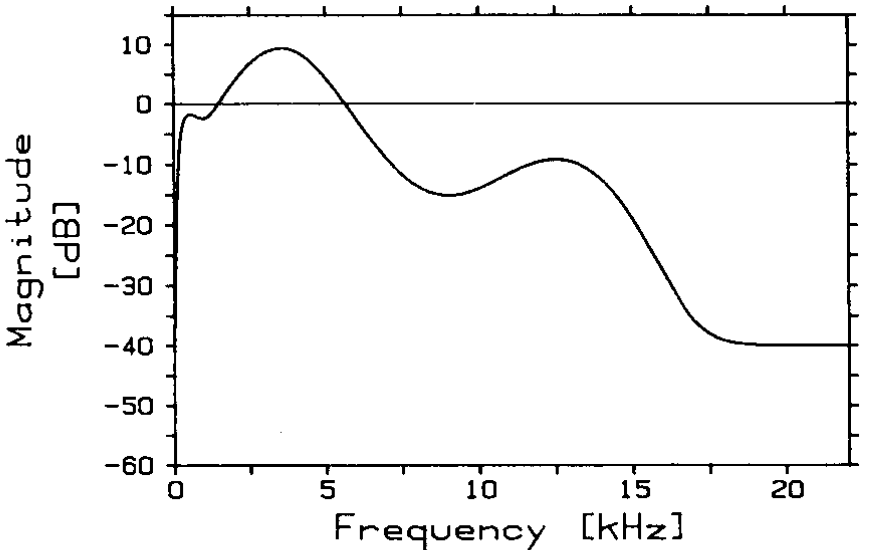
\includegraphics[scale=0.3]{Graph/NoiseShapingATH}
		\end{figure}
        plot from \footfullcite{wannamaker_psychoacoustically_1992}
	\end{frame}
	
	\begin{frame}{noise shaping}{dither \& noise shaping 1/3}
        \begin{figure}[!hbt]
			\begin{center}
	            \begin{picture}(120,40)
	
	                %boxes
	                \put(27,17){\dashbox (11,20){}}
	                \put(19,3){\framebox (6,6){\scriptsize{$z^{-1}$}}}
	
	                %lines horizontal
	                \put(0,20){\vector(1,0){10}}
	                \put(15,20){\vector(1,0){15}}
	                \put(35,20){\vector(1,0){15}}
	                \put(25,12){\vector(1,0){5}}
	                \put(40,12){\vector(-1,0){5}}
	                
	                \put(32.5,6){\vector(-1,0){7.5}}
	                \put(19,6){\line(-1,0){6.5}}
	
	                %lines vertical
	                \put(25,20){\line(0,-1){8}}
	                \put(40,20){\line(0,-1){8}}
	                \put(12.5,6){\vector(0,1){11.5}}
	                \put(32.5,9.5){\line(0,-1){3.5}}
	                
	                \put(32.5,30){\vector(0,-1){7.5}}

	                \put(12.5,30){\vector(0,-1){7.5}}
	                
	                %circles
	                \put(12.5,20){\circle{5}} \put(11,19){{{+}}}
	                \put(32.5,20){\circle{5}} \put(31,19){{{+}}}
	                \put(32.5,12){\circle{5}} \put(31,11){{{+}}}
	                
	                \put(25,20){\circle*{1}}
	                \put(40,20){\circle*{1}}
	
	                %text
	                \put(29,12.5){\footnotesize{\shortstack[c]{-}}}
	                \put(14,16){\footnotesize{\shortstack[c]{-}}}
	                \put(25,38){\footnotesize{\shortstack[c]{Quantizer}}}
	                \put(30,32){\footnotesize{\shortstack[c]{q(i)}}}
	                \put(0,22){\footnotesize{\shortstack[c]{x(i)}}}
	                \put(50,22){\footnotesize{\shortstack[c]{y(i)}}}
	                \put(10,32){\footnotesize{\shortstack[c]{d(n)}}}

	                \put(20,-5){\footnotesize{\shortstack[c]{System A}}}







	
	                %boxes
	                \put(87,17){\dashbox (11,20){}}
	                \put(79,3){\framebox (6,6){\scriptsize{$z^{-1}$}}}
	
	                %lines horizontal
	                \put(60,20){\vector(1,0){10}}
	                \put(75,20){\vector(1,0){5}}
	                \put(85,20){\vector(1,0){5}}
	                \put(95,20){\vector(1,0){15}}
	                \put(77.5,12){\vector(1,0){12.5}}
	                \put(100,12){\vector(-1,0){5}}
	                
	                \put(92.5,6){\vector(-1,0){7.5}}
	                \put(79,6){\line(-1,0){6.5}}
	
	                %lines vertical
	                \put(77.5,20){\line(0,-1){8}}
	                \put(100,20){\line(0,-1){8}}
	                \put(72.5,6){\vector(0,1){11.5}}
	                \put(92.5,9.5){\line(0,-1){3.5}}
	                
	                \put(92.5,30){\vector(0,-1){7.5}}

	                \put(82.5,30){\vector(0,-1){7.5}}
	                
	                %circles
	                \put(72.5,20){\circle{5}} \put(71,19){{{+}}}
	                \put(82.5,20){\circle{5}} \put(81,19){{{+}}}
	                \put(92.5,20){\circle{5}} \put(91,19){{{+}}}
	                \put(92.5,12){\circle{5}} \put(91,11){{{+}}}
	                
	                \put(77.5,20){\circle*{1}}
	                \put(100,20){\circle*{1}}
	
	                %text
	                \put(89,12.5){\footnotesize{\shortstack[c]{-}}}
	                \put(74,16){\footnotesize{\shortstack[c]{-}}}
	                \put(85,38){\footnotesize{\shortstack[c]{Quantizer}}}
	                \put(90,32){\footnotesize{\shortstack[c]{q(i)}}}
	                \put(60,22){\footnotesize{\shortstack[c]{x(i)}}}
	                \put(110,22){\footnotesize{\shortstack[c]{y(i)}}}
	                \put(80,32){\footnotesize{\shortstack[c]{d(n)}}}
	                
	                \put(80,-5){\footnotesize{\shortstack[c]{System B}}}
	
	            \end{picture}
			\end{center}
	    \end{figure}
	\end{frame}
	
	\begin{frame}{noise shaping}{dither \& noise shaping 2/3}
		System A
			\begin{eqnarray*}
				y(i) &=& [x(i) + d(n) -q(i-1)]_Q \nonumber\\
				&=& x(i)+d(n)-q(i-1)+q(i)
			\end{eqnarray*}
			\pause
			\begin{eqnarray*}
				Y(z) &=& X(z) - z^{-1}\cdot Q(z) + Q(z) + D(z)\nonumber\\
				&=& X(z) + (1-z^{-1})\cdot Q(z) + D(z)
			\end{eqnarray*}
	\end{frame}
	
	\begin{frame}{noise shaping}{dither \& noise shaping 3/3}
		System B
			\begin{eqnarray*}
				y(i) &=& [x(i) + d(n) - q(i-1) - d(n-1)]_Q \nonumber\\
				&=& x(i)-q(i-1)+q(i)-d(n-1)+d(n)
			\end{eqnarray*}
			\pause
			\begin{eqnarray*}
				Y(z) &=& X(z) - z^{-1}\cdot Q(z) + Q(z) - z^{-1}\cdot D(z) + D(z)\nonumber\\
				&=& X(z) + (1-z^{-1})\cdot (Q(z) + D(z))
			\end{eqnarray*}
	\end{frame}
	
	\begin{frame}{noise shaping}{noise shaping audio examples}
        \begin{itemize}
            \item   \unit[16]{bit}: \includeaudio{00_Master_16_bit}
            \item   \unit[8]{bit}: \includeaudio{01_Truncate_8_bit}
            \item   \unit[8]{bit} dither: \includeaudio{02_Standard_Dither_8_bit}
            \item   \unit[8]{bit} standard noise shaping: \includeaudio{03_Most_Widely_Known_8_bit}
            \item   \unit[8]{bit} powerful noise shaping: \includeaudio{04_Most_Powerful_8_bit}
        \end{itemize}
	\end{frame}
	
	\begin{frame}{noise shaping}{noise shaping spectrograms}
        \vspace{-4mm}
		\begin{figure}
			\centering
				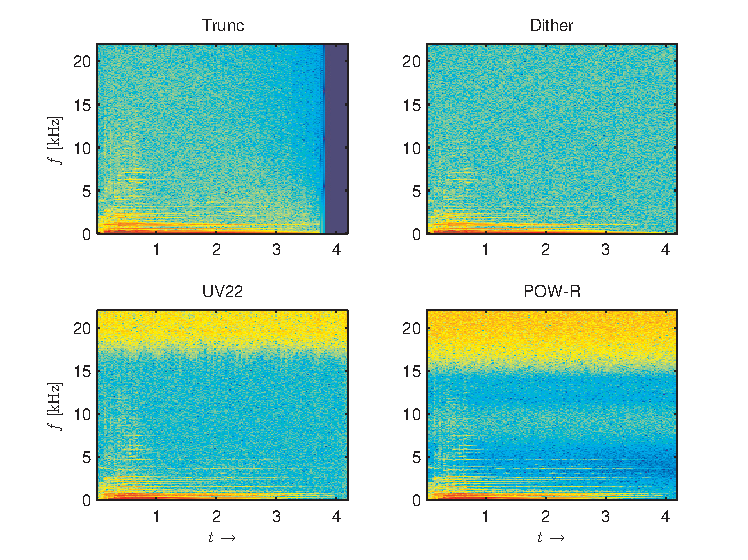
\includegraphics[scale=0.8]{Graph/noiseshaping_spectrum}
		\end{figure}
	\end{frame}
	
	\section{summary}	
		\begin{frame}{summary}{quantization: summary}
            \textit{three ways} of improving the (re-)quantization error
            \begin{itemize}
                \item   \textbf{oversampling}
                    \begin{itemize}
                        \item   reduces quantization error power in the audible band 
                        \item   \textit{process}: oversampling $\rightarrow$ filtering $\rightarrow$ downsampling
                    \end{itemize}
                \bigskip
                \item<2->   \textbf{dither}
                    \begin{itemize}
                        \item   reduces correlation of error and signal for low amplitude signals
                        \item   increases the power of the quantization error slightly
                        \item   \textit{process}: add triangular shaped low-level noise before word-length reduction
                    \end{itemize}
                \bigskip
                \item<3->   \textbf{noise-shaping}
                    \begin{itemize}
                        \item   reduces the audibility of the quantization error by shifting it to high frequencies 
                        \item   works best at high sample rates
                        \item   \textit{process}: feedback the quantization error
                    \end{itemize}
            \end{itemize}
		\end{frame}
 

\end{document}

